\chapter{Introduction}
\label{ch:intro}

Social insect societies are formed by thousands of individuals, which continuously move and interact with each other inside a dark nest. Honey bee colonies are thus organized complex and dynamical systems, which form a collective intelligence. Observing individual honey bees is, therefore, vital for understanding collective behavior, decision making, and organization of tasks within the colony.

Within the BeesBook project of the Biorobotics Lab of Freie Universität Berlin~\textcite{wario2015automatic} developed technologies to automatically track all individuals of a honey bee (Apis mellifera) colony. Shortly after birth, each bee has been marked on their thorax using circular 12-bit tags (figure~\ref{fig:markers}) and then added to the colony. The comb is observed by four cameras over a period of nine weeks and each picture is evaluated automatically. The resulting data set contains the position of each bee and its decoded id.

In this thesis, temporal interaction networks, based on spatial proximity, are derived from the described data set. Each node in the network is a bee and a link between two individuals is created if they share a position close to each other. Social network analysis methods are applied to determine the usefulness and the characteristics of the resulting networks and its communities.

Until now, social network analysis has been applied to only a subset of a honey bee colonies live, simply because the data were not available to this extent and quality so far.

\begin{figure}[htb]
	\centering
	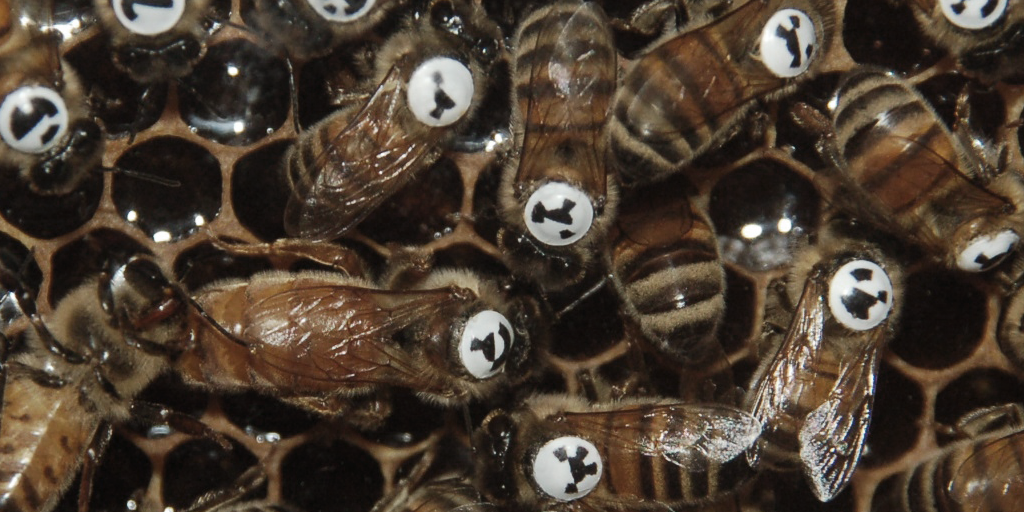
\includegraphics[width=1.0\textwidth]{Figures/markers}
	\caption{Tagged bees inside the hive.}
	\label{fig:markers}
\end{figure}

\section{Motivation}
Most of the studies in the field of animal social network analysis, especially when analysing the behaviour of social insects colonies, only include a reduced subset of the colonies life into analysis, due to the large number of individuals. Usually the reduction is carried out on three levels (1) time and resolution, (2) space, and (3) number of individuals.

\textcite{baracchi2014socio} observed 300 bees out of a colony with 4000 individuals over a peroid of 10 hours. One side of the hive was observed by taking a snapshot each minute. Coloured numbered discs were used for individually marking bees. \textcite{blonder2011time} colorpainted all individuals of ant colonies (size 6-90) and filmed the colonies for 30 minutes. Interactions between individuals were manually extracted by watching the videos. Labeling only a subset of the hive, a short observation period, and manually extracting information form photos or videos is very common in this field~\cite{naug2008structure, quevillon2015social}.

Using automated high resolution tracking data, which includes all individuals of the complete comb over a long time period allows for more advanced anaysis focusing on temporal dynamics. \textcite{mersch2013tracking} automatically tracked all individuals of six ant colonies over a period of 41 days. Applying the Infomap community detection algorithm to the physical contact networks for each day, revealed three distinct and robust groups. Each group represents a functional behavioural unit, with individuals changing groups as they age.

The majority of social insect interaction networks studies, due to previously technical limitations, aggregate temporal tacking data into single static networks.~\cite[Chapter~15]{krause2014animal} 


\section{Research Goal}

The aim of this thesis is to investigate whether the provided data set of tracked honey bees is useful for creating worker-worker interaction networks using spatial proximity as a proxy for interactions between bees. Thus, I need to implement a pipeline to infer networks out of the data set. Furthermore I want to find out if the resulting networks are suitable for social network analysis.

I want to achive my research goals by answering the following questions:

\begin{enumerate}
\item \emph{Is it possible to infer networks with the provided data set?}\\
What challenges and limitations does the data set imply?
\item \emph{What kind of networks emerge and what are their properties?}\\
How are those networks characterized and are they different from a random network? (structure and dynamics)
\item \emph{Do community structures exists?}\\
Are those communities robust?
\item \emph{How are those communities characterized?}\\
Do they reflect known colony behaviour in terms of age and spatial distribution?
\item \emph{How do the communities evolve over time?}\\
Are they stabel over time and how do members change communities over time? (dynamics)

\end{enumerate}


\section{Methodology}

Network Science Approach.

\section{Outline}
[TODO]